\documentclass[../sparc.tex]{subfiles}
\graphicspath{{\subfix{../images/}}}
\begin{document}

%%%%%%%%%%%%%%%%%%%%%%%%%%%%%%%%%%%%%%%%%%%%%%%%%%%%%%%%%%%%%%%%%%%%%%%%%%%%%%%%
\section{Графика}

Несмотря на то, что дисплей в нашем проекте используется текстовый, и он не даёт
нам возможности рисовать произвольные рисунки в любом месте экрана, нам доступна
возможность создавать собственные символы.  Эти символы затем можно отображать в
клетках дисплея.

Размер клетки на нашем дисплее составляет 8х5 пикселей (8 строк на 5 столбцов.)
Схематически это можно визуализировать, как показано на
рис. \ref{fig:game-dev-char}.

\begin{figure}[ht]
  \centering
  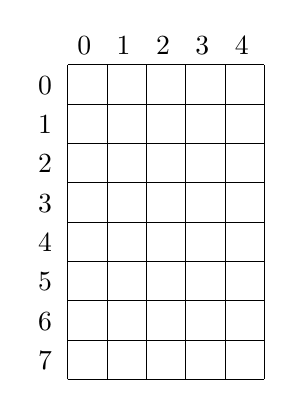
\begin{tikzpicture}
    \draw[step=0.5cm,black,very thin] (-2.5, -4) grid (0, 0);
    \foreach[count=\n from 0] \x in {-2.5, -2.0, ..., -0.5} {
      \draw (\x cm, 0) node[anchor=south west] {$\n$};
    }
    \foreach[count=\n from 0] \y in {-0.5, -1.0, ..., -4} {
      \draw (-3.0, \y) node[anchor=south west] {$\n$};
    }
  \end{tikzpicture}
  \caption{Схематическое изображение клетки, в которой отрисовывается символ.}
  \label{fig:game-dev-char}
\end{figure}

\end{document}
